
%(BEGIN_QUESTION)
% Copyright 2003, Tony R. Kuphaldt, released under the Creative Commons Attribution License (v 1.0)
% This means you may do almost anything with this work of mine, so long as you give me proper credit

Calculate all voltages, currents, and total power in this balanced Delta-Y system:

$$\includegraphics[width=15.5cm]{i02270x01.eps}$$

\begin{itemize}
\item{} $E_{line} =$
\vskip 10pt
\item{} $I_{line} =$
\vskip 10pt
\item{} $E_{phase(source)} =$
\vskip 10pt
\item{} $I_{phase(source)} =$
\vskip 10pt
\item{} $E_{phase(load)} =$
\vskip 10pt
\item{} $I_{phase(load)} =$
\vskip 10pt
\item{} $P_{total} =$
\end{itemize}

\vskip 20pt \vbox{\hrule \hbox{\strut \vrule{} {\bf Suggestions for Socratic discussion} \vrule} \hrule}

\begin{itemize}
\item{} Identify which fundamental principles of electric circuits apply to each step of your analysis of this circuit.  In other words, be prepared to explain the reason(s) ``why'' for every step of your analysis, rather than merely describing those steps.
\item{} Suppose the center of the wye-connected load were connected to earth ground.  Determine the amount of voltage between each vertex of the delta-connected source and earth ground.
\item{} Suppose one of the vertices of the delta-connected source were connected to earth ground.  Determine the amount of voltage between each terminal of the wye-connected load and earth ground.
\item{} Suppose one of the vertices of the delta-connected source were connected to earth ground.  Determine the amount of voltage between the center point of the wye-connected load and earth ground.
\end{itemize}


\underbar{file i02270}
%(END_QUESTION)





%(BEGIN_ANSWER)

\noindent
{\bf Partial answer:}

\begin{itemize}
\item{} $E_{line} =$ 2400 V
%\item{} $I_{line} =$ 4.619 A
%\item{} $E_{phase(source)} =$ 2400 V
\item{} $I_{phase(source)} =$ 2.667 A
%\item{} $E_{phase(load)} =$ 1385.6 V
\item{} $I_{phase(load)} =$ 4.619 A
%\item{} $P_{total} =$ 19.2 kW
\end{itemize}

%(END_ANSWER)





%(BEGIN_NOTES)

\begin{itemize}
\item{} $E_{line} =$ 2400 V
\item{} $I_{line} =$ 4.619 A
\item{} $E_{phase(source)} =$ 2400 V
\item{} $I_{phase(source)} =$ 4.619 A / $\sqrt{3}$ = 2.667 A
\item{} $E_{phase(load)} =$ 2400 V / $\sqrt{3}$ = 1385.6 V
\item{} $I_{phase(load)} =$ 1385.6 V / 300 $\Omega$ = 4.619 A
\item{} $P_{total} =$ ($\sqrt{3}$) (2400 V) (4.619 A) = 19.2 kW
\end{itemize}

%INDEX% Electronics review: 3-phase electrical power 

%(END_NOTES)


